\documentclass{article}
\usepackage{amsmath, sfmath, multicol, tkz-euclide, array, enumerate, tcolorbox, tabularray}
\renewcommand{\familydefault}{\sfdefault}
\setlength{\parindent}{0cm}
\pagestyle{empty}
\usepackage[left=1in, top=0.5in, right=1in, bottom=0.5in]{geometry}
\tikzset{>=stealth, label style/.append style={font=\footnotesize}}
\tcbset{colback=white}

\newcounter{example}[section]
\newenvironment{example}[1][]{\refstepcounter{example}\par\medskip
   {\color{red}\textbf{Example~\theexample. #1}}}{\medskip}

\begin{document}

\section*{Properties of Parallelograms}

\begin{tcolorbox}[colframe=orange!70!white, coltitle=black, title=\textbf{Today I Can}]
\begin{enumerate}
    \item Use properties of parallelograms to find unknown lengths and angle measures.
\end{enumerate}
\end{tcolorbox}
\bigskip 

\begin{tcolorbox}[colframe=black!20!white, opacitybacktitle=0.1, coltitle=black, title=\textbf{Parallelograms}]
A quadrilateral with 2 pairs of opposite parallel sides. \newline 

\begin{minipage}{0.5\textwidth}
\begin{itemize}
    \item $\overline{AB} \parallel \overline{CD}$
    \item $\overline{BC} \parallel \overline{AD}$
\end{itemize}
\end{minipage}
\begin{minipage}{0.4\textwidth}
    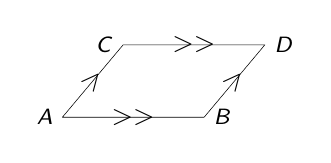
\begin{tikzpicture}[scale=0.6, decoration={markings,
mark=at position 0.5 with {\arrow[scale=2]{>}};}]
    \tkzDefPoints{0/0/A, 3/0/B}
    \tkzDefShiftPoint[A](50:2){C}
    \tkzDefShiftPoint[B](50:2){D}
    \tkzDrawPolygon(A,B,D,C)
    \tkzLabelPoints[left](A, C)
    \tkzLabelPoints[right](B, D)
    \tkzDefMidPoint(A,B) \tkzGetPoint{e}
    \node at (e) {$>>$};
    \tkzDefMidPoint(C,D) \tkzGetPoint{f}
    \node at (f) {$>>$};
    \tkzDefMidPoint(A,C) \tkzGetPoint{g}
    \node at (g) [rotate=50] {$>$};
    \tkzDefMidPoint(B,D) \tkzGetPoint{h}
    \node at (h) [rotate=50] {$>$};
    \end{tikzpicture}
\end{minipage}
\end{tcolorbox}

\textsc{Parallelograms} 

\begin{itemize}
    \item Opposite sides are parallel
    \item Opposite sides are congruent
    \item Opposite angles are congruent
    \item Consecutive angles are supplementary
    \item Diagonals bisect each other
\end{itemize}

\begin{example}
Find the value of $x$ in each parallelogram.
\begin{multicols}{2}
\begin{enumerate}[(a)]
    \item \mbox{}  
    \item \mbox{}
\end{enumerate}
\end{multicols}
\begin{minipage}{0.5\textwidth}
    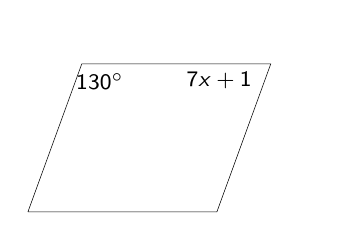
\begin{tikzpicture}[scale=0.8]
    \tkzDefPoints{0/0/A, 3/0/B}
    \tkzDefShiftPoint[A](70:2.5){D}
    \tkzDefShiftPoint[B](70:2.5){C}
    \tkzDrawPolygon(A,B,C,D)
    \tkzLabelAngle[pos=-1, yshift=0.25cm](B,C,D){\footnotesize $7x+1$}
    \tkzLabelAngle[pos=0.5, yshift=0.1cm](A,D,C){\footnotesize $130^\circ$}
    \end{tikzpicture}
\end{minipage}
\begin{minipage}{0.4\textwidth}
    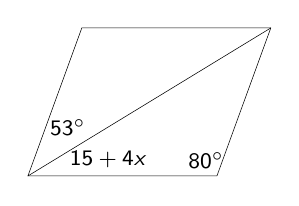
\begin{tikzpicture}[scale=0.8]
    \tkzDefPoints{0/0/A, 3/0/B}
    \tkzDefShiftPoint[A](70:2.5){D}
    \tkzDefShiftPoint[B](70:2.5){C}
    \tkzDrawPolygon(A,B,C,D)
    \tkzDrawSegment(A,C)
    \tkzLabelAngle[xshift=0.25cm](B,A,C){\footnotesize $15+4x$}
    \tkzLabelAngle[](C,A,D){\footnotesize $53^\circ$}
    \tkzLabelAngle[pos=0.3](C,B,A){\footnotesize $80^\circ$}
    \end{tikzpicture}
\end{minipage}

\vspace{1in}

\begin{multicols}{2}
\begin{enumerate}[(a)]  \setcounter{enumi}{2}
    \item \mbox{} 
    \item $BE=20, \quad BD=6x+4$
\end{enumerate}
\end{multicols}
\begin{minipage}{0.5\textwidth}
    \begin{tikzpicture}[scale=0.8]
    \tkzDefPoints{0/0/A, 3/0/B}
    \tkzDefShiftPoint[A](70:2.5){D}
    \tkzDefShiftPoint[B](70:2.5){C}
    \tkzDrawPolygon(A,B,C,D)
    \tkzLabelSegment[below](A,B){11}
    \tkzLabelSegment[above](C,D){$2x+5$}
    \end{tikzpicture}
\end{minipage}
\begin{minipage}{0.4\textwidth}
    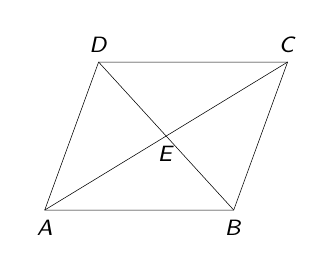
\begin{tikzpicture}[scale=0.8]
    \tkzDefPoints{0/0/A, 3/0/B}
    \tkzDefShiftPoint[A](70:2.5){D}
    \tkzDefShiftPoint[B](70:2.5){C}
    \tkzDrawPolygon(A,B,C,D)
    \tkzDrawSegments(A,C B,D)
    \tkzInterLL(A,C)(B,D)
    \tkzGetPoint{E}
    \tkzLabelPoints[below](A,B,E)
    \tkzLabelPoints[above](C,D)
    \end{tikzpicture}
\end{minipage}
\end{example}

\newpage 

\begin{example}
Verify that each of the following are parallelograms.

\begin{enumerate}[(a)]
    \item $A(5, \, 4), \, B(3, \, -6), \, C(0, \, -10), \, D(2, \, 0)$ \newline
    
    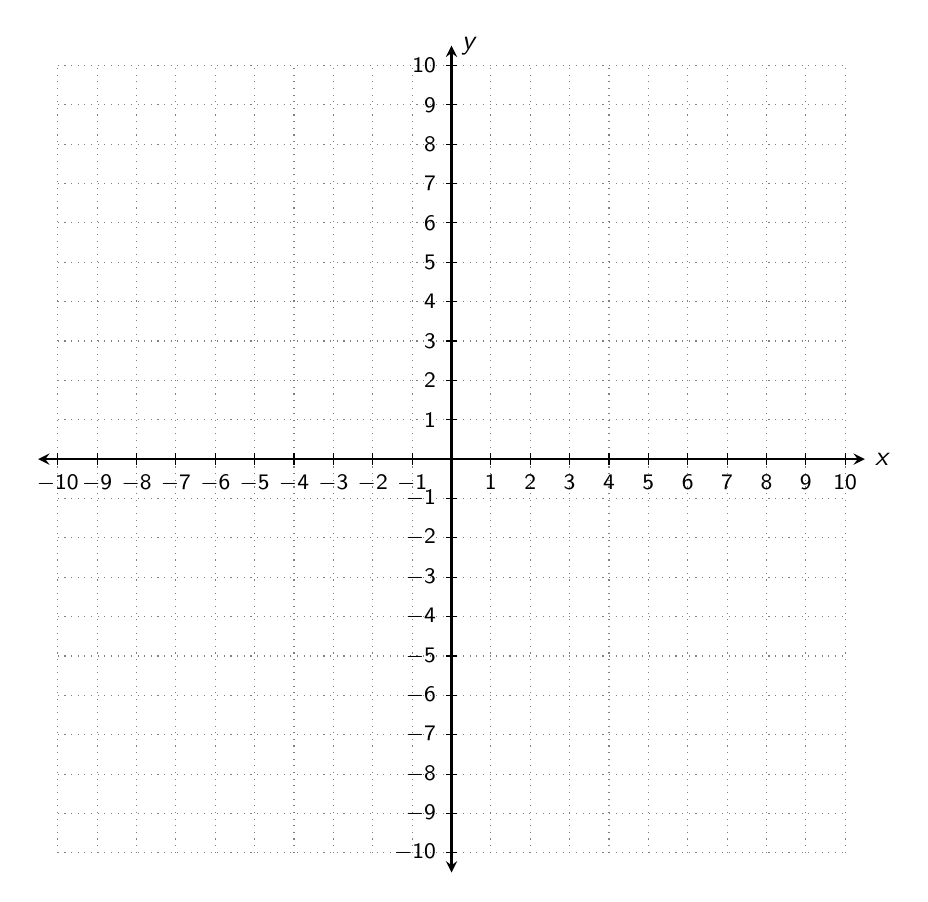
\begin{tikzpicture}[scale=0.5]
    \draw [gray, dotted] (-10,-10) grid (10,10);
    \draw [<->, thick] (-10.5,0) -- (10.5,0) node [right] {$x$};
    \foreach \x in {-10,...,-1,,1,...,10}
    \draw (\x, 0.15) -- (\x, -0.15) node [below] {\footnotesize $\x$};
    \draw [<->, thick] (0,-10.5) -- (0,10.5) node [right] {$y$};
    \foreach \y in {-10,...,-1,,1,...,10}
    \draw (0.15,\y) -- (-0.15, \y) node [left] {\footnotesize $\y$};
    \end{tikzpicture}
    
    \vfill 
    
    \item $A(-5, \, -2), \, B(-3, \, 4), \, C(3, \, 1), \, D(1, \, -5)$ \newline
    
    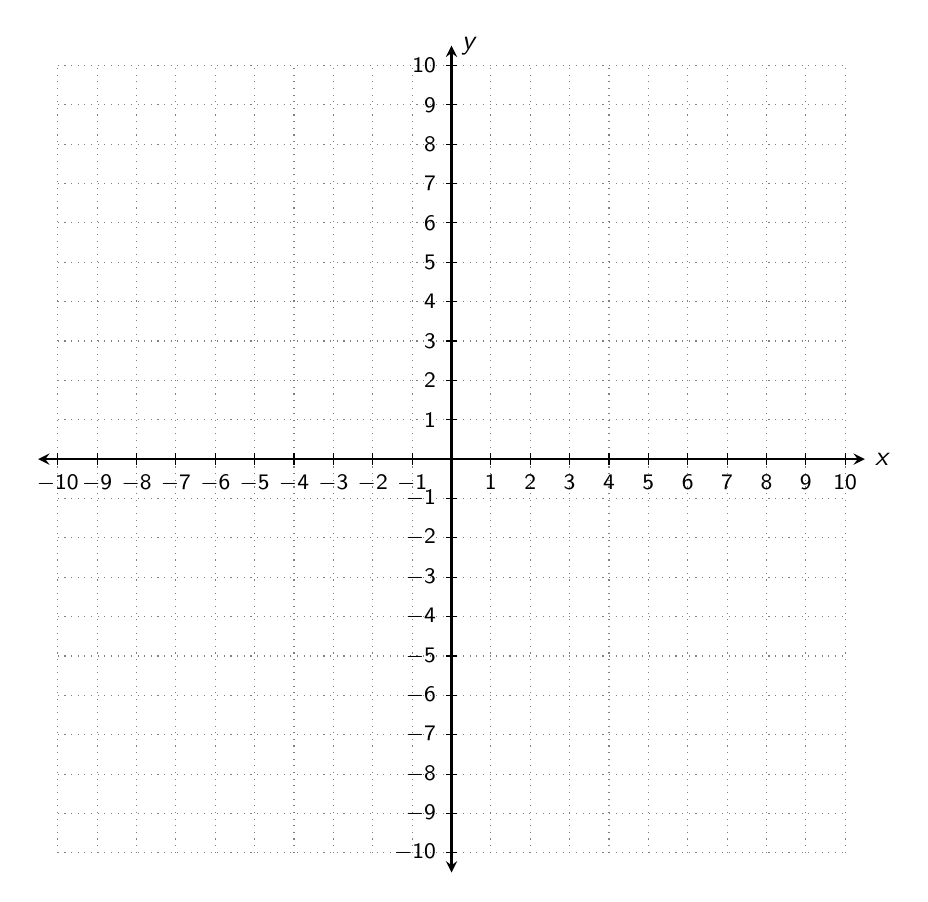
\begin{tikzpicture}[scale=0.5]
    \draw [gray, dotted] (-10,-10) grid (10,10);
    \draw [<->, thick] (-10.5,0) -- (10.5,0) node [right] {$x$};
    \foreach \x in {-10,...,-1,,1,...,10}
    \draw (\x, 0.15) -- (\x, -0.15) node [below] {\footnotesize $\x$};
    \draw [<->, thick] (0,-10.5) -- (0,10.5) node [right] {$y$};
    \foreach \y in {-10,...,-1,,1,...,10}
    \draw (0.15,\y) -- (-0.15, \y) node [left] {\footnotesize $\y$};
    \end{tikzpicture}
\end{enumerate}
\end{example}

\end{document}
